\documentclass{article}
\usepackage[utf8]{inputenc}
\usepackage{tabularx} % extra features for tabular environment
\usepackage{amsmath}  % improve math presentation
\usepackage{graphicx} % takes care of graphic including machinery
\usepackage{xspace}
\usepackage{tikz}
\usepackage{pdfpages}
\usepackage{enumitem}
\usetikzlibrary{babel}
\usepackage[american]{circuitikz}
\usetikzlibrary{calc}
\usepackage{float}
\usepackage{siunitx}
\usepackage{pgfplots}
\usepackage[skins,theorems]{tcolorbox}
\tcbset{highlight math style={enhanced,
  colframe=red,colback=white,arc=0pt,boxrule=1pt}}
\pgfplotsset{width=10cm,compat=1.9}
\usepackage[margin=1in,letterpaper]{geometry} % decreases margins
\usepackage{cite} % takes care of citations
\usepackage[final]{hyperref} % adds hyper links inside the generated PDF file
\hypersetup{
colorlinks=true,       % false: boxed links; true: colored links
linkcolor=blue,        % color of internal links
citecolor=blue,        % color of links to bibliography
filecolor=magenta,     % color of file links
urlcolor=blue        
}

\begin{document}

\title{{\textbf{ASSIGNMENT 6}}}
\author{\textbf{TADIPATRI UDAY KIRAN REDDY}\\\textbf{EE19BTECH11038}}
\maketitle

\section*{\hfil Problem 1}
\begin{figure}[H]
	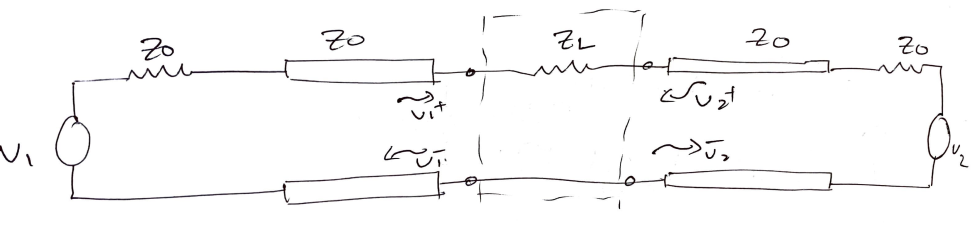
\includegraphics[scale=0.5]{./figs/q1.png}
\end{figure}
\subsection*{$V_{2}^+ = 0$}
\begin{gather}
\Gamma _{L1} = \frac{\frac{Z_L+Z_0}{Z_0}-1}{\frac{Z_L+Z_0}{Z_0}+1} = \frac{Z_L}{Z_L + 2Z_0}\\
\implies \frac{V_1^-}{V_1^+} = \tcbhighmath[drop fuzzy shadow]{S_{11} = \frac{Z_L}{Z_L + 2Z_0}}
\end{gather}

Since source at Port 2 is matched network then,
\begin{gather}
V_2^- = (V_1^+ + V_1^-)\frac{Z_0}{Z_0 + Z_L}\\
\frac{V_2^- }{V_1^+} = S_{12} = (S_{11} + 1)\frac{Z_0}{Z_0 + Z_L}\\
\implies S_{12} = \tcbhighmath[drop fuzzy shadow]{\frac{2Z_0}{Z_L + 2Z_0}}
\end{gather}
\subsection*{$V_{1}^+ = 0$}
The above network is clearly symetric which scattering matrix is symetric.
\begin{equation}
\tcbhighmath[drop fuzzy shadow]{\mathbf{S} = \begin{bmatrix}
\frac{Z_L}{Z_L + 2Z_0} & \frac{2Z_0}{Z_L + 2Z_0}\\
\frac{2Z_0}{Z_L + 2Z_0} & \frac{Z_L}{Z_L + 2Z_0}
\end{bmatrix}}
\end{equation}
In this case we get,
\begin{equation}
\tcbhighmath[drop fuzzy shadow]{\mathbf{S} = \begin{bmatrix}
0.0476 & 0.9524\\
0.9524 & 0.0476
\end{bmatrix}}
\end{equation}
\section*{\hfil Problem 2}
\subsection*{(a)}
\begin{figure}[H]
	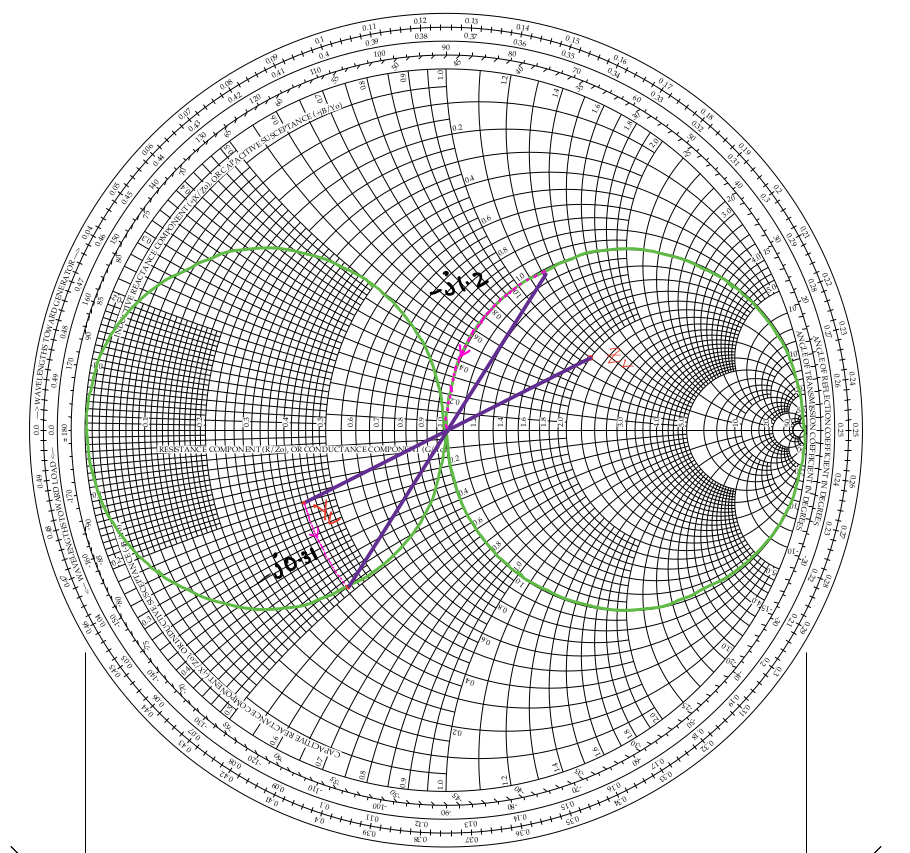
\includegraphics[scale=0.5]{./figs/q2_s.png}
\end{figure}
\begin{figure}[H]
	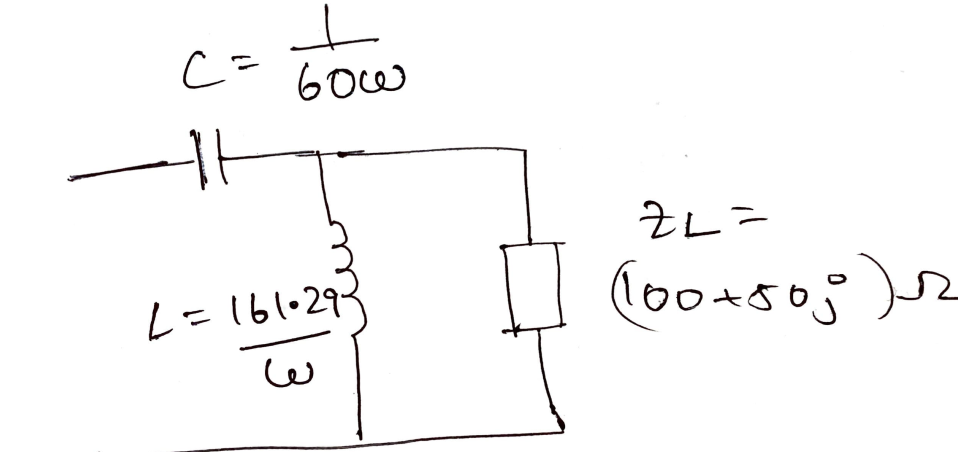
\includegraphics[scale=0.3]{./figs/q2a.png}
\end{figure}
\subsection*{(b)}
\begin{figure}[H]
	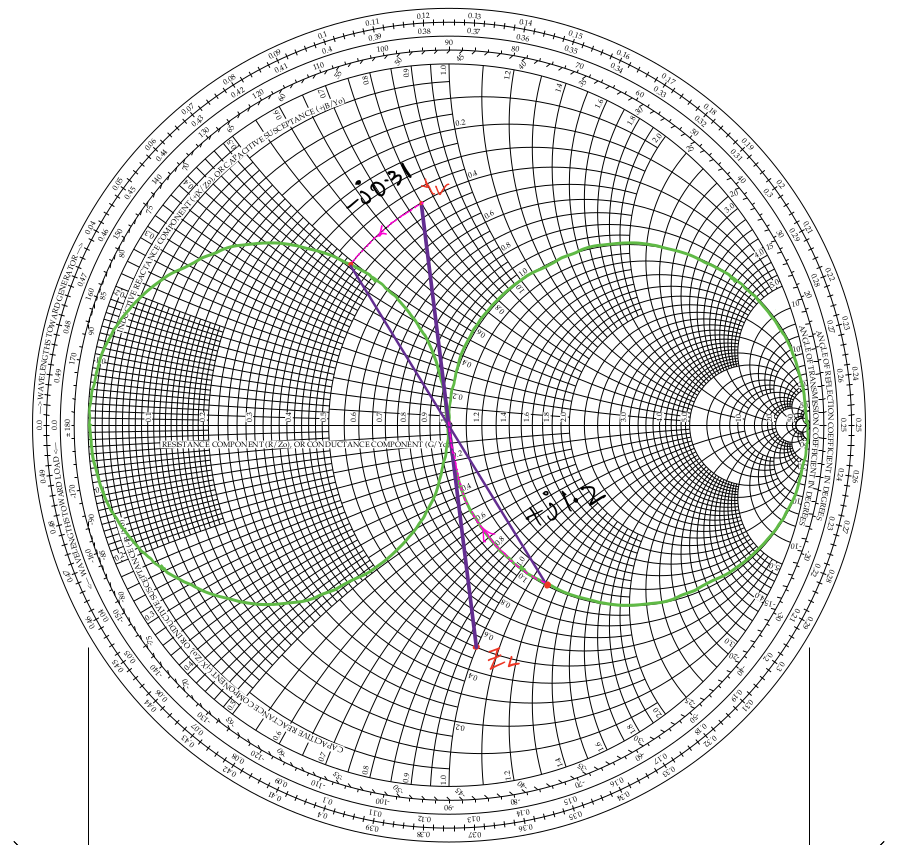
\includegraphics[scale=0.5]{./figs/q2b_s.png}
\end{figure}
\begin{figure}[H]
	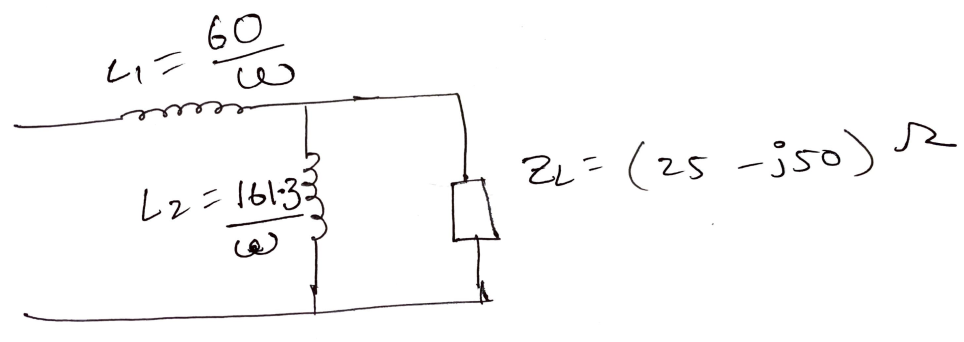
\includegraphics[scale=0.3]{./figs/q2b.png}
\end{figure}

\section*{\hfil Problem 3}
At DC we see that $Z_{in} = Z_L = 50 \si{\ohm}$ which means the line is lossless $\implies \alpha = 0$.\\
At 1GHz when lossless,
\begin{gather}
	Z_{in}(x) = Z_0\left[\frac{Z_L + Z_0jtan(\beta _{1GHz}l)}{Z_0 - jZ_Ltan(\beta _{1GHz}l)}\right]\\
	4 = z_0\left[\frac{1 + z_0jtan(\beta _{1GHz}l)}{z_0 - jtan(\beta _{1GHz}l)}\right]\\
	\implies 3z_0 - j\left(tan(\beta _{1GHz}l)[z_0^2 + 4]\right) = 0
\end{gather}
The above equation is valid iff $z_0 = 0$ and $\beta _{1GHz}l = n\pi$. This means that,
\begin{gather}
z_0 = \frac{1}{50}\sqrt{\frac{L_0}{C_0}} = 0\\
2\pi.10^9.\sqrt{L_0C_0}l = n\pi
\end{gather}
The above two equation implies that $\tcbhighmath[drop fuzzy shadow]{L_0 = 0}$.
\begin{gather}
\tcbhighmath[drop fuzzy shadow]{Z_0 = 0 \si{\ohm};
t_{PD} = 0 s}
\end{gather}
\end{document}